% flashcards-title: Metric unit conversion map
% flashcards-desc: Arrows connect kilograms to grams by times one thousand and meters to centimeters by times one hundred, with reverse division arrows.
\documentclass[dvisvgm,tikz,border=8pt]{standalone}\usetikzlibrary{arrows.meta,patterns}

\definecolor{qraNavy}{HTML}{17324D}
\definecolor{qraBlue}{HTML}{2B6CB0}
\definecolor{qraGold}{HTML}{B7791F}
\definecolor{qraPale}{HTML}{EAF2F8}
\definecolor{qraGray}{HTML}{5C6773}

\tikzset{
  qra axis/.style={draw=qraNavy, line width=1.2pt},
  qra tick/.style={draw=qraNavy, line width=1pt},
  qra guide/.style={draw=qraGray, densely dashed, line width=0.8pt},
  qra counter/.style={circle, draw=qraNavy, fill=qraPale, line width=0.9pt, minimum size=7mm, inner sep=0pt},
  qra label/.style={font=\sffamily\bfseries, text=qraNavy},
  qra small label/.style={font=\sffamily, text=qraNavy},
}

\begin{document}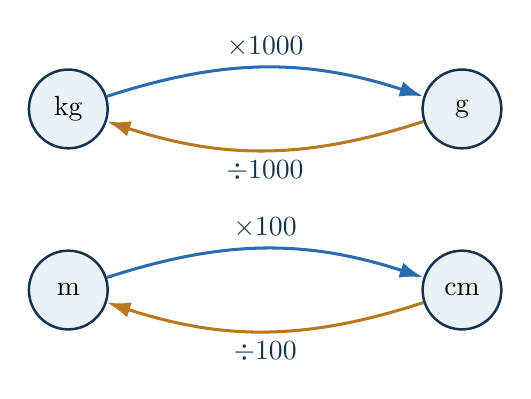
\begin{tikzpicture}[x=1cm,y=1cm]
\node[qra counter,minimum size=10mm](kg)at(0,2.3){kg};\node[qra counter,minimum size=10mm](g)at(5,2.3){g};
\draw[qraBlue,line width=1.1pt,-{Latex[length=3mm,width=2mm]}](kg)to[bend left=18]node[qra small label,above]{\(\times1000\)}(g);
\draw[qraGold,line width=1.1pt,-{Latex[length=3mm,width=2mm]}](g)to[bend left=18]node[qra small label,below]{\(\div1000\)}(kg);
\node[qra counter,minimum size=10mm](m)at(0,0){m};\node[qra counter,minimum size=10mm](cm)at(5,0){cm};
\draw[qraBlue,line width=1.1pt,-{Latex[length=3mm,width=2mm]}](m)to[bend left=18]node[qra small label,above]{\(\times100\)}(cm);
\draw[qraGold,line width=1.1pt,-{Latex[length=3mm,width=2mm]}](cm)to[bend left=18]node[qra small label,below]{\(\div100\)}(m);
\end{tikzpicture}\end{document}
